\documentclass[beamer]{standalone}

\usepackage{tikz}

\usetikzlibrary{backgrounds}
\usetikzlibrary{calc}
\usetikzlibrary{positioning}

\definecolor{x-red}{HTML}{e41a1c}
\definecolor{x-blue}{HTML}{3694E0}
\definecolor{x-green}{HTML}{63E05F}
\definecolor{x-purple}{HTML}{D365E3}
\definecolor{x-orange}{HTML}{E8A100}
\definecolor{x-yellow}{HTML}{fff200}

\definecolor{almost-white}{HTML}{f0f0f0}


\begin{document}

\begin{standaloneframe}

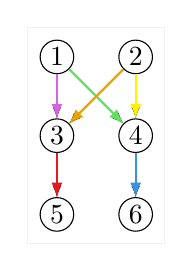
\begin{tikzpicture}[
    node/.style={draw, circle,
        inner sep=.05cm,
    },
    wire/.style={-latex},
    background rectangle/.style={ draw=almost-white, line width=0pt, },
    show background rectangle,
]

% half adder
\node [node] (a) at (0,2) {\(1\)};
\node [node] (b) at (1,2) {\(2\)};
\node [node] (xor1) at (0,1) {\(3\)};
\node [node] (and1) at (1,1) {\(4\)};
\node [node] (s) at (0,0) {\(5\)};
\node [node] (cout) at (1,0) {\(6\)};


\onslide<1>{
    \draw [wire] (a) to (xor1);
    \draw [wire] (a) to (and1);
    \draw [wire] (b) to (xor1);
    \draw [wire] (b) to (and1);
    \draw [wire] (xor1) to (s);
    \draw [wire] (and1) to (cout);
}

% colored
\onslide<2>{
    \draw [wire, x-purple, thick] (a) to (xor1);
    \draw [wire, x-green, thick] (a) to (and1);
    \draw [wire, x-orange, thick] (b) to (xor1);
    \draw [wire, x-yellow, thick] (b) to (and1);
    \draw [wire, x-red, thick] (xor1) to (s);
    \draw [wire, x-blue, thick] (and1) to (cout);
}

\end{tikzpicture}


\end{standaloneframe}

\end{document}
